	\documentclass[a4paper,12pt]{article}
%%%%%%%%%%%%%%%%%%%%%%%%%%%%%%%%%%%%%%%%%%%%%%%%%%%%%%%%%%%%%%%%%%%%%%%%%%%%%%%%%%%%%%%%%%%%%%%%%%%%%%%%%%%%%%%%%%%%%%%%%%%%%%%%%%%%%%%%%%%%%%%%%%%%%%%%%%%%%%%%%%%%%%%%%%%%%%%%%%%%%%%%%%%%%%%%%%%%%%%%%%%%%%%%%%%%%%%%%%%%%%%%%%%%%%%%%%%%%%%%%%%%%%%%%%%%
\usepackage{eurosym}
\usepackage{vmargin}
\usepackage{amsmath}
\usepackage{graphics}
\usepackage{framed}
\usepackage{epsfig}
\usepackage{subfigure}
\usepackage{enumerate}
\usepackage{fancyhdr}

\setcounter{MaxMatrixCols}{10}
%TCIDATA{OutputFilter=LATEX.DLL}
%TCIDATA{Version=5.00.0.2570}
%TCIDATA{<META NAME="SaveForMode"CONTENT="1">}
%TCIDATA{LastRevised=Wednesday, February 23, 201113:24:34}
%TCIDATA{<META NAME="GraphicsSave" CONTENT="32">}
%TCIDATA{Language=American English}

\pagestyle{fancy}
\setmarginsrb{20mm}{0mm}{20mm}{25mm}{12mm}{11mm}{0mm}{11mm}
\lhead{MS4222} \rhead{Kevin O'Brien} \chead{Sampling} %\input{tcilatex}

\begin{document}




\section*{Tutorial Sheet 4}
\begin{enumerate}

    
    \item


The data set X and Y are both assumed to be normally distributed. A graphical procedure was carried out to assess whether or not this assumption of normality is valid for data set Y. Consider the Q-Q plot in the figure below.
\begin{enumerate}[(a)]
\item Provide a brief description on how to interpret this plot.
\item What is your conclusion for this procedure? Justify your answer.
\end{enumerate}

	
	\begin{center}
		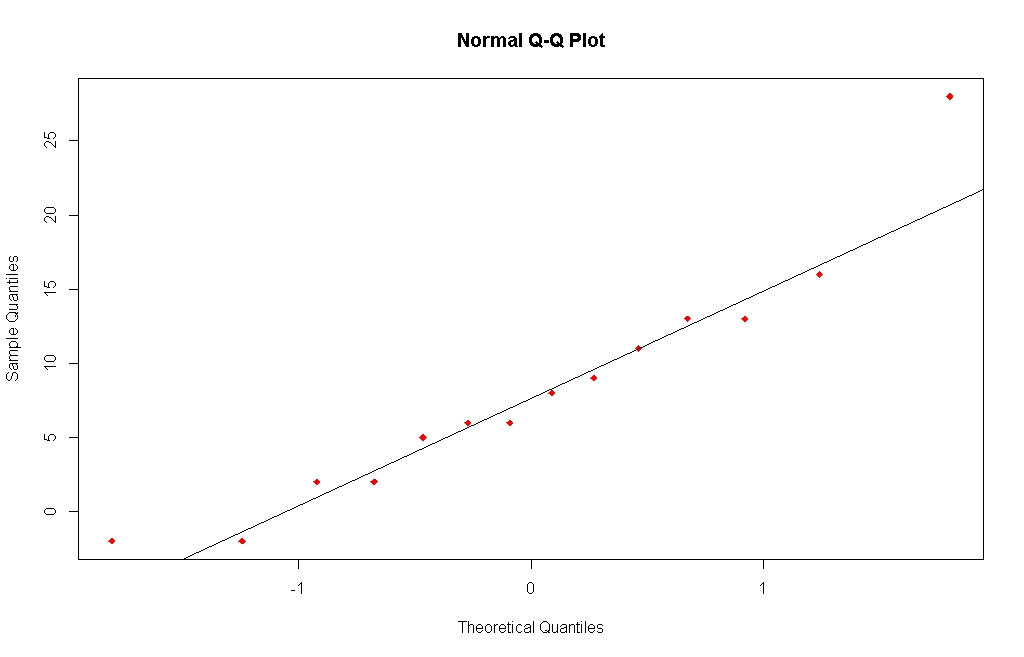
\includegraphics[scale=0.445]{images/10AQQplot}
	\end{center}
	
	%----------------------------------------------------------%

    \item

The standard deviations of data sets X and Y are given in the R code below. An inference procedure was carried out to assess whether or not X and Y can be assumed to have equal variance.
The standard deviation of X is 3.11.The standard deviation of Y is 1.89

\begin{enumerate}[(i)]
\item Formally state the null and alternative hypothesis.
\item The test statistic has been omitted from the R code output. Compute the value of the test statistic.
\item What is your conclusion for this procedure? Justify your answer.
\item Explain how a conclusion for this procedure can be based on the 95\% confidence interval.
\end{enumerate}
\begin{framed}
\begin{verbatim}
> var.test(X,Y)

     F test to compare two variances

data:  X and Y 
F = ………, num df = 13, denom df = 11, p-value = 0.1078
alternative hypothesis: true ratio of variances is not equal to 1 
95 percent confidence interval:
 0.7951967 8.6239382 

sample estimates:
ratio of variances 
          ……… 
\end{verbatim}
\end{framed}


\item 
The following statistical procedure is based on this dataset.
\begin{center}
\begin{tabular}{|cccc|}
	\hline
	% after \\: \hline or \cline{col1-col2} \cline{col3-col4} ...
	6.98 &8.49 &7.97& 6.64\\
	8.80 &8.48 &5.94& 6.94\\
	6.89 &7.47 &7.32& 4.01\\
	\hline
\end{tabular}
\end{center}

\begin{framed}

	\begin{verbatim}
	> grubbs.test(x, two.sided=T)
	
	Grubbs test for one outlier
	
	data:  x
	G = 2.4093, U = 0.4243, p-value = 0.05069
	alternative hypothesis: lowest value 4.01 is an outlier
	\end{verbatim}
\end{framed}

\begin{enumerate}[(i)]
	\item Describe what is the purpose of this procedure. State the null and alternative hypothesis.
	\item Write the conclusion that follows from it.
	\item State any relevant assumptions for this procedure.
\end{enumerate}

\end{enumerate}
\end{document}
